\chapter{Introduction} \label{chap:introduction}
%================================================================================%
\section{Context} \label{sec:introduction:context}
% 1) 2 paragraphes maximum sur l'évolution des IHMs
Since the advent of computers, significant effort has been invested in improving how they interface with humans, fostered by continuous technological improvements through the 20th and 21st centuries.
%
In the mid-20th century, computers were still large, costly, and highly specialized tools mostly reserved for big institutions and companies. The emergence of high-level programming languages vastly simplified the work of researchers at these institutions by enabling them to create complex algorithms without having to manipulate individual bits. 
%
From the 1970s onward, the user base of computers gradually expanded to cover a broader segment of society. As they became accessible to more people, more intuitive methods of interaction were required, leading to the emergence of graphical user interfaces (GUIs).
%
Thanks to GUIs, various tasks became accessible to less tech-savvy users, such as writing text and manipulating images.
%
The early 21st century saw the use of computers and small portable electronic devices explode thanks in part to massive improvements in efficiency, performance, size, and cost. 
%
This rapid digitalization of our world could leave vulnerable people, such as the elderly, at risk of being shut out from the rest of society. Now more than ever, it is essential to design computer systems with accessibility in mind so that no one is left behind: technology can, and should, be at the service of everyone, regardless of their age, ethnicity, and whether they suffer from a disability or not. Only that way could society truly benefit from the new possibilities offered by the digitization of many of its facets, including healthcare, education, culture, and governance.

% 2) Gesture interfaces
Fortunately, the increase in computing power and improvements in sensing devices opened up a wealth of new possibilities for human-computer interaction (HCI). 
In particular, 3D gesture-based interfaces have been proposed as a natural and intuitive alternative to traditional input methods~\cite{Vatavu:2014b,Huang:2019}, typically relying on vision-based sensors, like the Leap Motion Controller (LMC) and Microsoft Kinect, or wearable devices, like smart rings~\cite{Gheran:2018}, smartwatches, and armbands, to capture user motion.
% 
Each sensor has some advantages and limitations regarding, \eg cost, performance, privacy, and practicality, which make them more suitable for different applications. 
%
For instance, vision-based sensors can accurately track user motion from a distance~\cite{Weichert:2013,DeSmedt:2017}, but are sensitive to occlusion and lighting conditions, have a limited field of view, and may raise some privacy concerns.  
%
Wearable devices, while exempted from these issues, are more intrusive as they must be worn by the user during interaction, thus making them less suitable for public spaces.

% 3) Radars for gesture recognition
Radar sensors~\cite{Yeo:2016} have emerged as a promising alternative to these technologies. They combine a compact form factor and low power consumption with the ability to capture gestures through opaque surfaces and in challenging lighting conditions, all while preserving user privacy. These characteristics could make them well-suited for gestural interaction in public spaces.
%
Radars have been successfully applied in various domains, including virtual reality~\cite{Huesser:2021}, activity recognition~\cite{Avrahami:2018,Avrahami:2020}, material recognition~\cite{Flintoff:2018, Yeo:2016}, and tangible interaction~\cite{Yeo:2019}. 
%
However, research on radar-based gestural interfaces is still in its early stages and presents several challenges.
%
In particular, the lack of consensus on a few affordable and efficient off-the-shelf radar sensors has resulted in a plethora of (custom) radar systems, often incompatible with each other.
%
This is especially problematic, as existing works typically rely on sophisticated deep-learning algorithms for gesture recognition to cope with the complexity of radar signals. These algorithms are usually tailored to a specific sensor and gesture set, which complicates their (re)use in actual applications.

% 4) This research in 1 or 2 sentences
In light of this context, this thesis aims to advance the state of radar-based gesture interaction by providing tools and methods that bridge the gap between researchers and practitioners to facilitate the development of highly usable radar-based gesture interfaces.



%================================================================================%
\section{Research} \label{sec:introduction:research}

%--------------------------------------------------------------------------------%
\subsection{Statement and Research Questions} \label{sec:introduction:research:research-questions}
Radars have many advantages over other devices, such as vision-based sensors. Provided that developers and practitioners can overcome their limitations, radar sensors may become one of the keys to building ubiquitous gesture interaction, such as envisioned by \c{S}iean \etal~\cite{Siean:2023}.
%
However, research on radar-based gestural interfaces is in its infancy and many challenges that hinder their seamless integration and widespread adoption still have to be solved.

The central objective of this thesis is thus twofold: (1) {explore the use of radar for gesture recognition} and (2) {provide tools and methods to facilitate the development of highly usable (radar-based) gesture interfaces}. 
%
We further break down this objective into five research questions (RQs):
\begin{enumerate}[label=\textit{RQ\arabic*}]
    \item \textit{What are the main challenges of mid-air gesture recognition?} 
    Developers and practitioners may face multiple challenges in the development of gesture-based applications. It thus is crucial to identify these challenges as a first step towards fostering the development of gestural interaction.
    \item \textit{What is the performance of radar sensors for mid-air gesture recognition?} 
    Evaluating the efficacy and efficiency of radar-based gesture recognition will enable us to identify the scenarios in which radars could be a relevant alternative to other types of sensors. In addition, it would help us identify avenues for improving their performance, \eg by applying signal processing.
    \item \textit{What types of gesture-based applications would benefit from radar sensors?} 
    Despite their limitations, radars have many advantages over other sensors, such as their ability to sense gestures through opaque surfaces and in various lighting conditions, which could them more suitable for specific applications depending on the kind of performance that they offer. The answer to RQ2 will help us answer this research question as well.
    \item \textit{How can we foster collaboration between researchers and practitioners working on (radar) gesture recognition?}
    Fostering collaboration, \eg by facilitating the sharing of data and algorithms, has many benefits for both the scientific community and practitioners. It reduces the necessary steps to repeat and replicate experiments, which are major pillars of the scientific method, encourages building upon previous research (\eg to improve an existing algorithm), and makes this research more readily available to use in real-world applications.
    \item \textit{How can tools and methods aid in designing gesture-based applications that operate independently of gesture recognition logic?} 
    Separating the gesture recognition logic from the user interface of an application enables developers to focus on polishing the actual user experience and facilitates future modifications to the gesture recognition logic, \eg to support new sensors, change the gesture set, or improve the gesture recognition algorithm. Developing appropriate tools and methods is thus paramount to encourage the development of highly usable gesture-based interfaces. 
\end{enumerate}

%--------------------------------------------------------------------------------%
\newpage
\subsection{Scope}
We define the scope of this thesis as follows:
\begin{enumerate}[label=\textit{S\arabic*}]
    \item \textit{Use off-the-shelf sensors}: relying on off-the-shelf sensors ensures that our findings can be easily reproduced and replicated by other researchers.
    \item \textit{Use existing gesture recognizers}: relying on existing gesture recognizers allows us to follow a more generic approach, with the goal of providing useful tools and methods that are compatible with many techniques for gesture recognition.
    \item \textit{Focus on mid-air arm and hand gestures}: mid-air gestures promise natural interaction~\cite{Wigdor:2011} with a very large degree of freedom, but can be challenging to recognize with radar systems due to the small surface area of the hand. Focusing on mid-air gestures is a good starting point towards supporting more types of gestures, such as breathing patterns or even tongue gestures.
    \item \textit{Focus on non-critical applications}: as radar-based gesture recognition is still in its infancy, we will mostly focus on non-critical applications, such as multimedia applications, which do not require infallible gesture recognition.
    \item \textit{Support user customization}: our tools and methods should support user-defined gestures, as they can result in higher memorability and an overall more enjoyable experience compared to pre-defined gesture sets~\cite{Nacenta:2013}. In addition, custom gestures can make applications more accessible for users with disabilities.
\end{enumerate}
We will also strive to produce software that satisfies at least four of the ISO/IEC 25010 software quality properties~\cite{iso25010}, namely:
\begin{enumerate}[label=\textit{P\arabic*}]
    \item \textit{Compatibility}: defined as the ``degree to which a product, system or component can exchange information with other products, systems or components, and/or perform its required functions while sharing the same hardware or software environment''~\cite{iso25010}.
    \item \textit{Maintainability}: defined as the ``degree of effectiveness and efficiency with which a product or system can be modified to improve it, correct it or adapt it to changes in environment, and in requirements''~\cite{iso25010}.
    \item \textit{Portability}: defined as the ``degree of effectiveness and efficiency with which a system, product or component can be transferred from one hardware, software or other operational or usage environment to another''~\cite{iso25010}.
    \item \textit{Usability}: defined as the ``degree to which a product or system can be used by specified users to achieve specified goals with effectiveness, efficiency, and satisfaction in a specified context of use''~\cite{iso25010}.
\end{enumerate}

%--------------------------------------------------------------------------------%
\subsection{Contributions}
% Contributions
This thesis makes several contributions to the field of gesture recognition in the form of literature reviews, tools, methods, applications, datasets, and experiments.

\subsubsection{Literature Reviews}
A targeted literature review (TLR)~\cite{Kysh:2013} and two systematic reviews of the literature (SLR)~\cite{Kitchenham:2010} were conducted to gather insight into the state of research in the field of (radar-based) gesture interaction:
\begin{itemize}
    \item \textit{TLR on gestural interaction}: a summary of the literature on the topic of gesture-based interaction in general, including gesture elicitation studies, the challenges of gesture recognition, and examples of gesture-based interfaces.
    \item \textit{SLR on LMC-based gesture interaction}: a look into how the LMC, a relatively mature vision-based sensor for gesture interaction, was used by researchers and practitioners to implement gesture recognition.
    \item \textit{SLR on radar-based gesture recognition}: a deep dive into the state of radar-based gesture recognition in the literature that focuses on applications, radar systems, gestures, and algorithms.
\end{itemize}

\subsubsection{Tools and Methods}
We provide two tools and one method that aims at fostering the development of highly usable (radar-based) gesture interfaces:
\begin{itemize}
    \item \textit{\ql framework}: a tool that addresses most of the challenges usually faced when creating gestural interfaces and provides an easy way to evaluate and compare gesture recognition algorithms. Its modular architecture featuring standardized modules facilitates the sharing of algorithms, sensors, and datasets across researchers and practitioners.
    \item \textit{User-centered development method}: an iterative development method and evaluation protocol for gestural interfaces that guide developers through the design process of highly usable gesture-based applications.
    \item \textit{Radar data pre-processing pipeline}: an electromagnetic model and inversion-based approach that normalizes radar signal to become independent from the radar system and background scene.
\end{itemize}

\subsubsection{Applications}
We developed one gesture-based application in the context of this thesis, but many more were built by other developers using \ql (see Section~\ref{sec:quantumleap:integration}): 
\begin{itemize}
    \item \textit{Large User Interface}: a gesture-based application that enables the manipulation of multimedia content with hand gestures and serves as a demonstration of the \ql framework and our user-centered development method.
\end{itemize}

\subsubsection{Datasets and Experiments}
Three experiments were conducted, each with its corresponding dataset, to evaluate the performance of our radar data pre-processing pipeline on a wide range of gestures performed by multiple users in different contexts.
These datasets allow the testing and comparison of gesture recognition techniques under various conditions and will thus be made publicly available to foster research and development in the field of gesture recognition.
\begin{itemize}
    \item \textit{Sensors comparison}: a dataset featuring 16 gesture classes from one participant recorded with three different devices, including two radars and an LMC. The corresponding experiment compares the performance of the three sensors in various testing configurations.
    \item \textit{20 gestures}: a dataset featuring 20 gesture classes from six participants recording with a Walabot sensor. The corresponding experiment evaluates the suitability of radar sensors for recognizing large sets of gestures and identifies smaller subsets of highly-differentiable gestures.
    \item \textit{Gestures through materials}: a dataset featuring nine gesture classes from 20 participants recorded with a Walabot through three types of materials (wood, PVC, and glass). The corresponding experiment investigates the performance of the Walabot when sensing gestures through materials and the ability of our pre-processing pipeline to normalize radar data sensed through different materials.
\end{itemize}


%================================================================================%
\section{Overview of the Thesis} \label{sec:introduction:overview}
\fig~\ref{fig:graphical-summary} provides a graphical overview of this thesis. Subsequent tasks are represented from top to bottom, along with their related chapter(s), contribution(s), and research question(s). Each chapter may cover one or more research question(s), contribution(s), and task(s).

\subsubsection{Chapter~\ref{chap:state_of_the_art}: State of the Art} 
This chapter positions this work in the literature by exploring the state of the art. 
%
We first provide an overview of gesture-based interaction, including gesture elicitation studies, the technical challenges of building gestural interaction, and examples of applications.
%
We then conduct a first SLR focusing on the Leap Motion Controller (LMC), a relatively mature vision-based sensing technology, to help contextualize the current state of radar-based gesture recognition.
%
With this context in mind, we conduct a second SLR that covers radar-based gesture interaction in general, including applications, sensors, gestures, and algorithms for gesture recognition.
%
We then conclude this chapter by relating the current state of the art to this work's context and objectives. 

\subsubsection{Chapter~\ref{chap:quantumleap}: Facilitating the Development of Gesture-based Applications} 
In this chapter, we introduce \ql, a software tool that attempts to address most of the challenges usually faced when creating gestural interfaces, to foster the development of new gesture-based applications.
%
We first provide an overview of the tool's modular architecture, designed to enable the reuse of components across applications.
%
We then conduct an experiment to evaluate the usability of \ql among seven software developers of various experience levels.
%
Finally, we explore recent projects that utilized and/or extended the \ql framework and we discuss its advantages and limitations.

\subsubsection{Chapter~\ref{chap:quantumleap-testing}: Streamlining the Evaluation of Gesture Recognizers} 
In this chapter, we introduce the \ql testing tool, an extension to \ql that allows researchers and practitioners to evaluate the performance of gesture recognizers, \eg to compare them against the current state of the art or to select an adequate recognizer for a specific application. The tool reuses the standardized components of \ql to facilitate sharing modules, testing procedures, and results.
%
We explain how we integrated the tool into \ql, present its main features, including its supported testing procedures, configuration user interface, and results format, and discuss its advantages and limitations.

\subsubsection{Chapter~\ref{chap:lui}: Designing Highly Usable Gesture-based Applications} 
In this chapter, we propose a user-centered iterative development method and evaluation protocol for gesture-based interfaces, which aims to support the development of highly usable gestural interfaces.
%
We detail how we applied the method and evaluation protocol to a real use-case scenario: the development of an application for manipulating multimedia objects on large displays with hand gestures. 

\subsubsection{Chapter~\ref{chap:radar-challenges}: Addressing the Challenges of Radar-based Gesture Recognition} 
In this chapter, we introduce a full-wave electromagnetic model and inversion-based approach for radar signal processing that aims to overcome the challenges of radar sensors for gesture recognition so that developers and practitioners can take full advantage of their capabilities.
%
We first lay the theoretical groundwork for the data processing pipeline and then provide information about each of its six stages and their effect on the radar signal.

\subsubsection{Chapter~\ref{chap:radar-experiments}: Experimenting with Radar-based Gestures}
In this chapter, we investigate the efficacy of our new radar signal processing approach by conducting three different experiments: (1) comparing the performance of radar-based and vision-based sensors on the same set of gestures, (2) evaluating the efficacy of our pipeline on a large set of gestures performed by multiple users and on smaller, highly differentiable subsets, and (3) investigating whether gestures can be accurately recognized when captured through three different types of materials and the ability of our pipeline to normalize their signal.
%
We first describe each sensor, as well as the recording procedure and pre-processing applied to each dataset. 
%
We then provide information about the testing procedure of each experiment, discuss their results, and consider their implications for the design of radar-based gestural interfaces.

% \subsubsection{Chapter~\ref{chap:zerog}: TODO.} 
% This chapter

\subsubsection{Chapter~\ref{chap:conclusion}: Conclusion} 
In this last chapter, we conclude this thesis by summarizing our work and discussing future avenues for research.

\begin{figure}
    \centering
    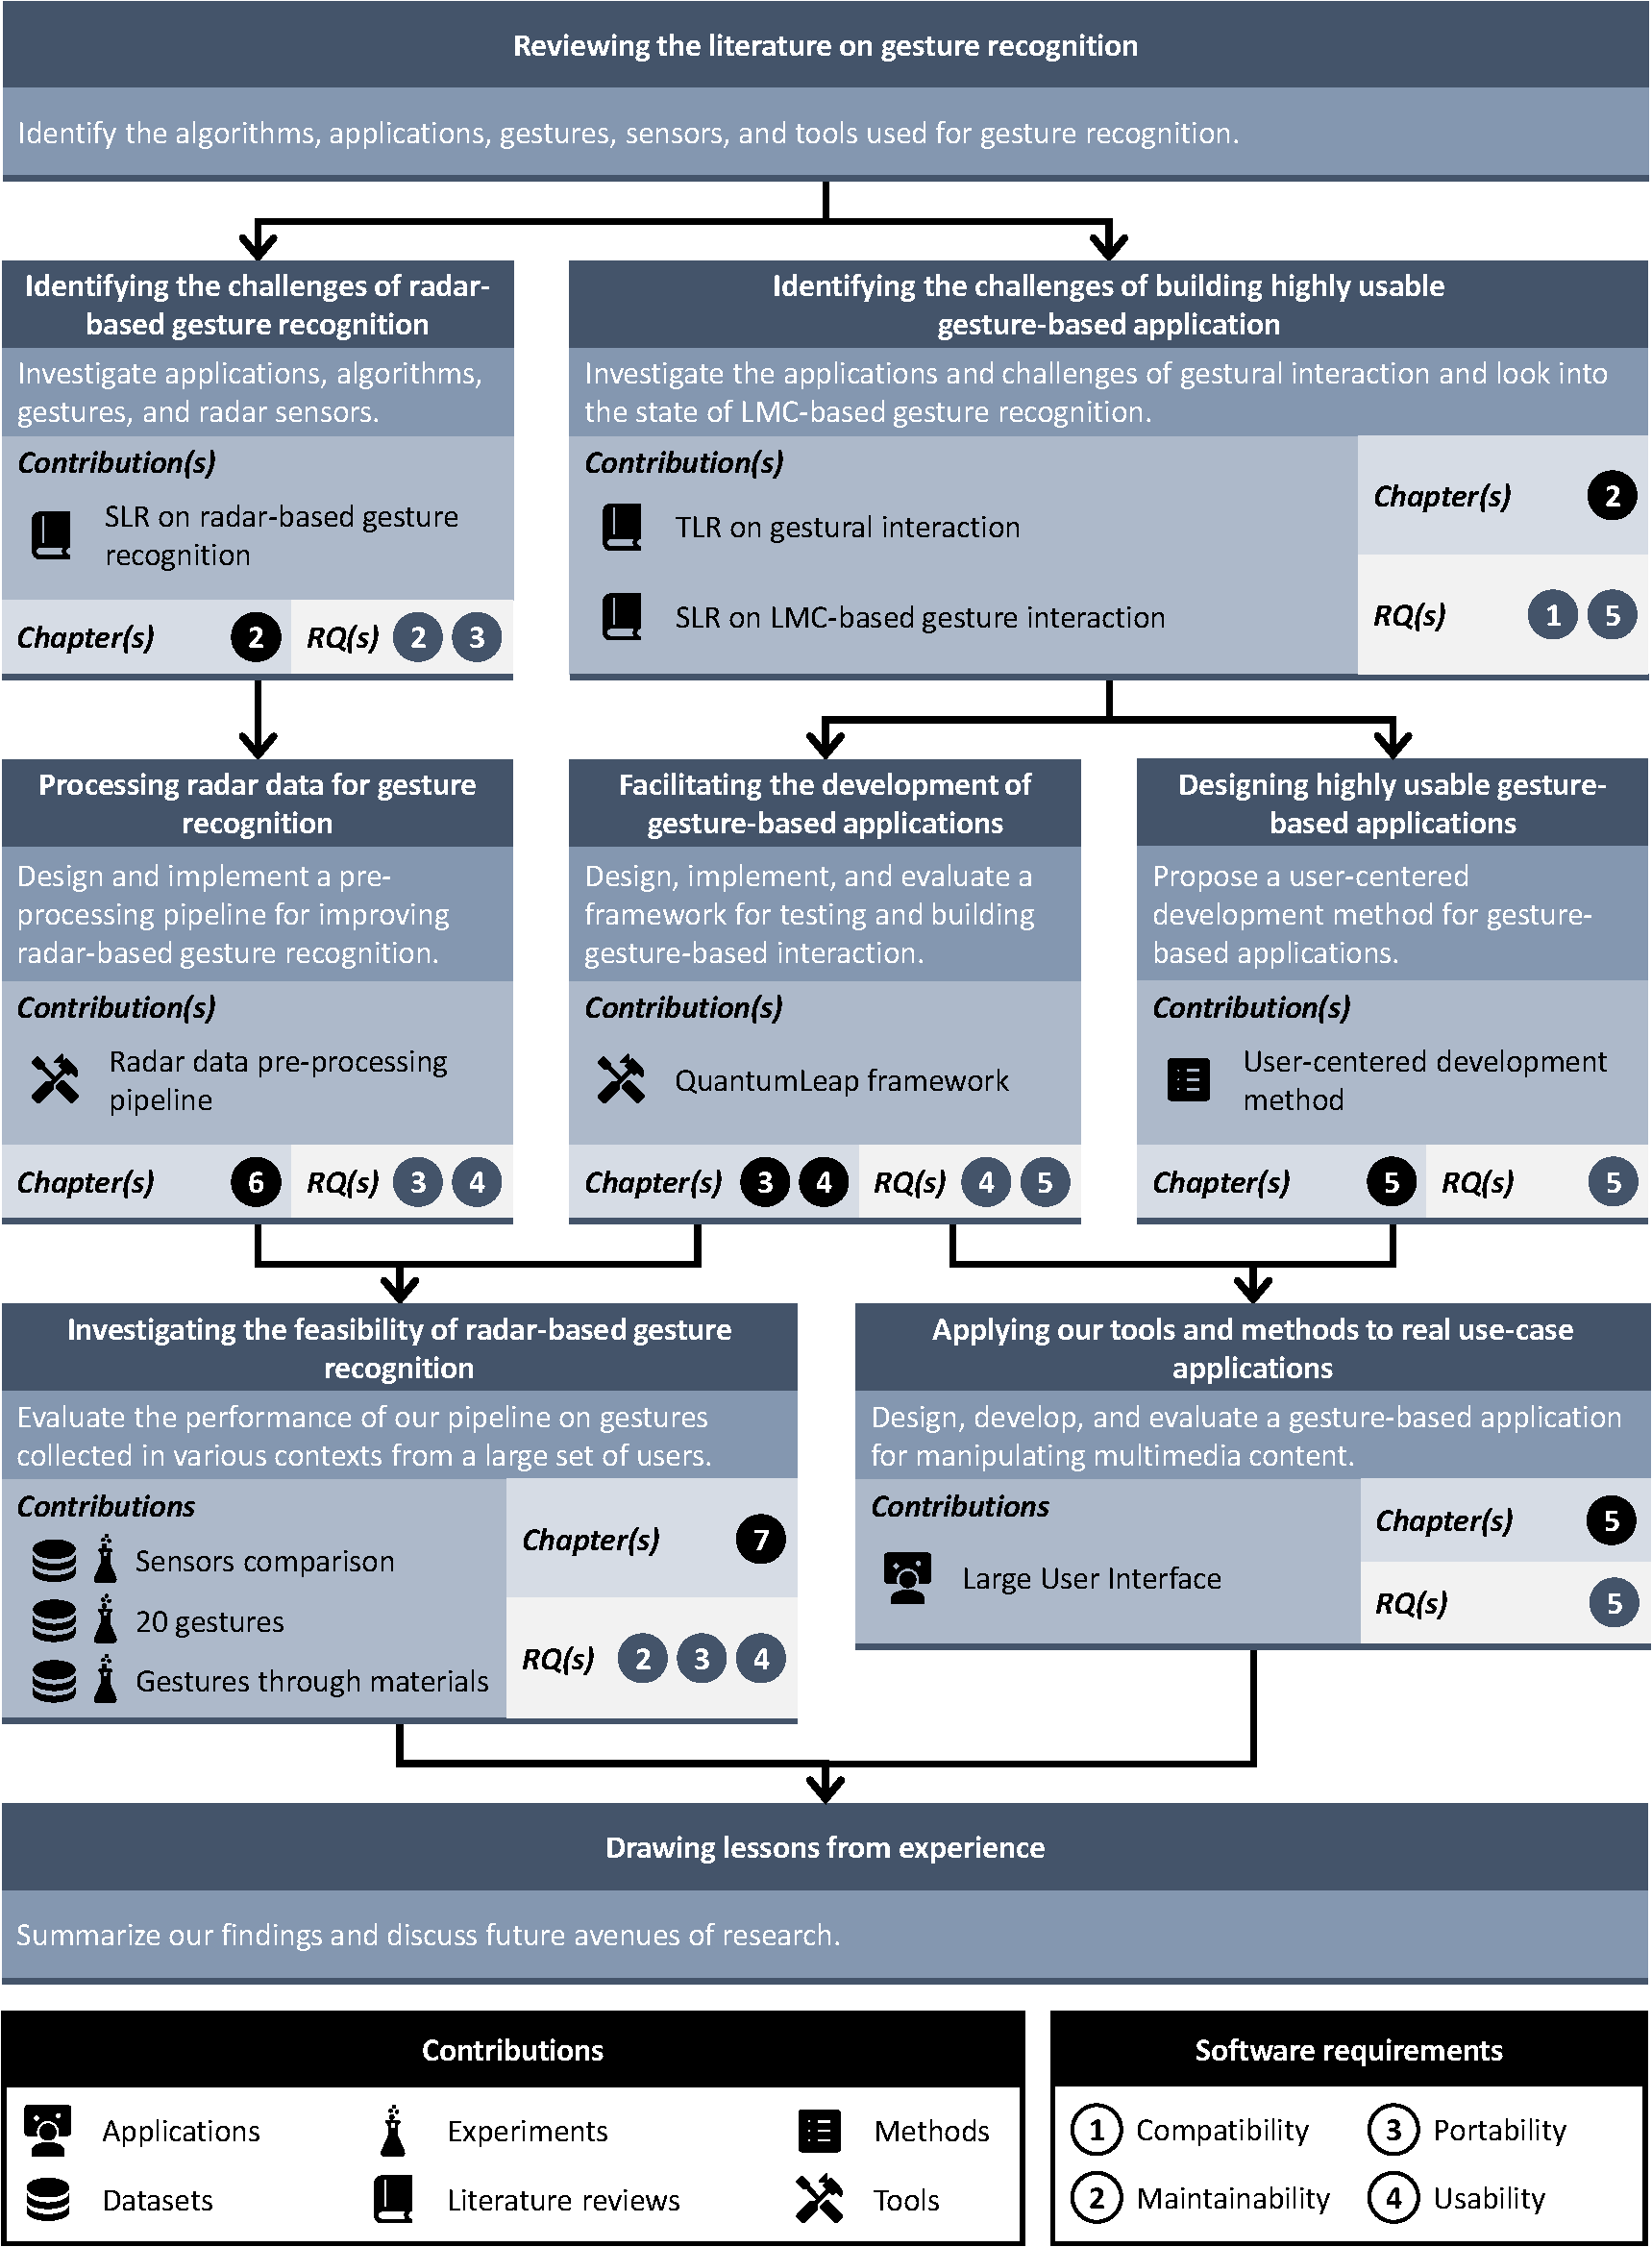
\includegraphics[width=\linewidth]{Figures/Introduction/graphical-summary.pdf}
    \vspace{-18pt}
    \caption{Overview of our research method. For each task, we provide the related contribution(s), chapter(s), and research question(s) (RQ).}
    \label{fig:graphical-summary}
\end{figure}
